% -*- mode : latex; coding: utf-8 -*-
\chapter{Background} \label{sec:backgrounds}

\section{Compute Express Link (CXL)}
Compute Express Link (CXL) is coherency and memory semantics on top of the PCIe 5.0 \cite{PCIe} based IO semantics. PCIe is a layered protocol that defines data exchange between peripheral devices, CPU and memory \cite{PCIe-simulation}. PCIe consists of physical, data link, transaction layers. PCIe interconnection consists of multiple point-to-point links between a pair of devices \cite{PCIe}. Each link can be broken down into one or more lanes. Each lane consists of two pairs of differential signaling wires one pair for transmission in each direction \cite{PCIe-simulation}. Each lane is capable of transmitting data at a rate of 4GB/s in PCIe 5.0. Also, PCIe is a packet-based protocol that packets are exchanged between devices. Since CXL is built on top of PCIe 5.0, CXL also consists of point-to-point links between a pair of devices (processor-accelerator, processor-memory deivce) and exchange data in the format of packet. In CXL, three protocols (CXL.io, CXL.cache, CXL.mem) are dynamically multiplexed. By using three protocols, CXL maintains unified, coherent memory space between CPU and any memory on the attached CXL device. This protocol reduces software stack complexity, device cost and complexity since CXL solves all the coherency related issues.

\begin{figure}[ht]
  \centering
  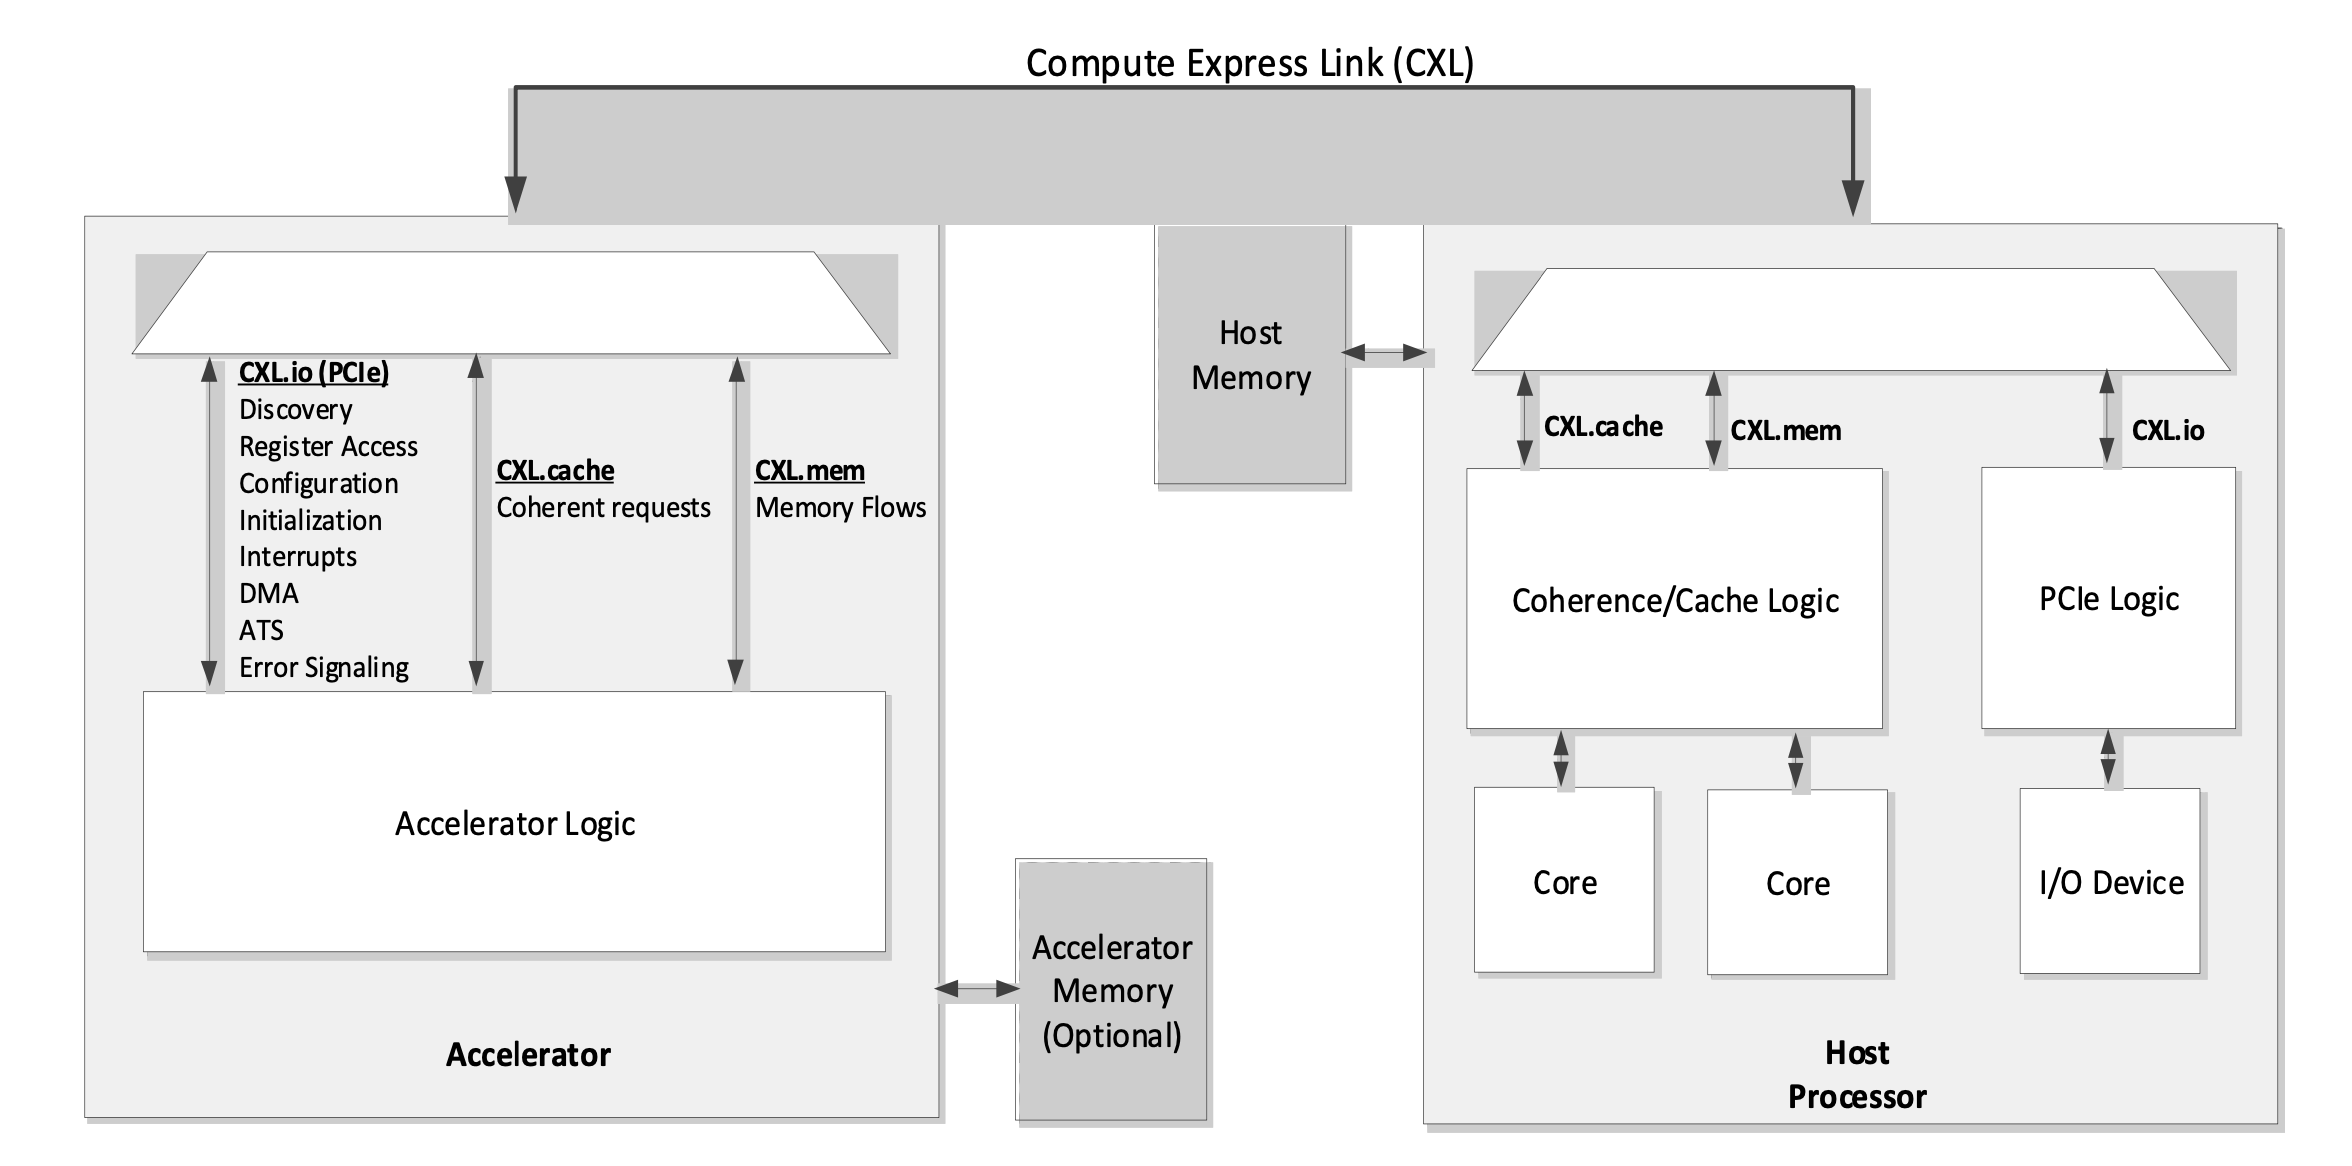
\includegraphics[width=\textwidth]{figures/cxl-overview.png}
  \caption{Conceptual diagram of accelerator attached to processor via CXL.}
  \label{fig:cxl-overview}
\end{figure}

Figure \ref{fig:cxl-overview} shows the conceptual diagram of accelerator attached to processor via CXL. CXL.io is almost almost identical to PCIe. It's used for discovery, register access, configuration, etc. CXL.cache is mainly about coherency. It is used to send and receive coherent requests. CXL.cache helps CXL device to access host processor's memory coherently. CXL.mem deals with memory requests and responds. This protocol helps host processor to access CXL attached memory.

\begin{figure}[ht]
  \centering
  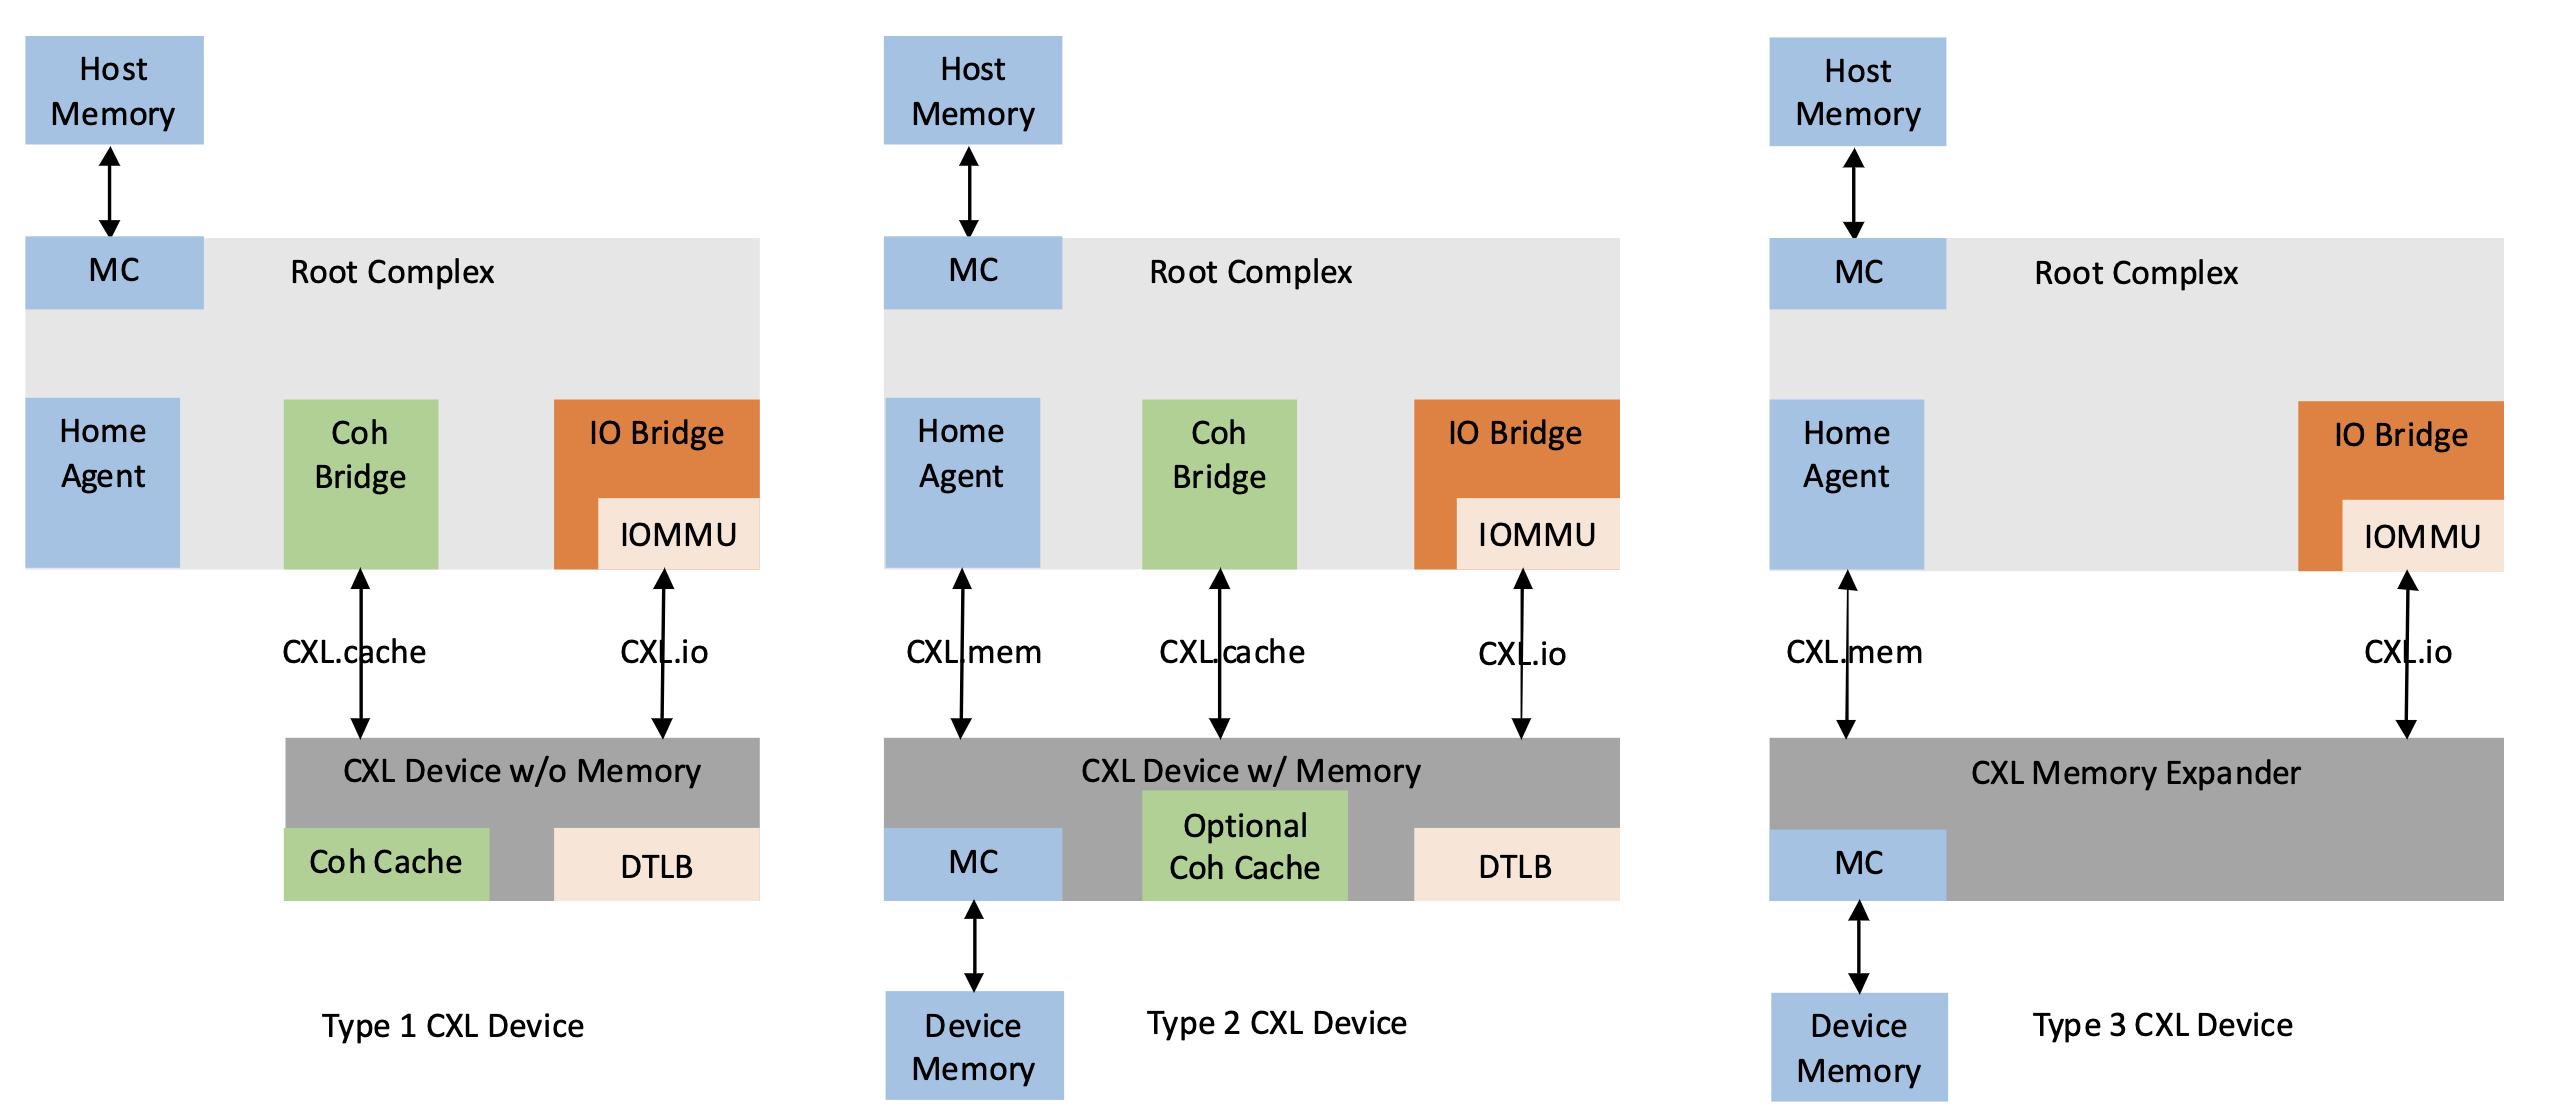
\includegraphics[width=\textwidth]{figures/cxl-device-type.png}
  \caption{Three possible CXL device types.}
  \label{fig:cxl-device-type}
\end{figure}

Figure \ref{fig:cxl-device-type} shows three different types of CXL device by combining three protocols. Type 1 device uses CXL.io and CXL.cache. This enables CXL device to have fully coherency with host memory. CXL.io helps detecting the device and performing initialization. CXL.cache gives CXL device a chance to access host memory coherently. Type 2 device adds coherent CXL device on top of type 1 device. Thus, type 2 device uses all three protocols (CXL.io, CXL.cache, CXL.mem).  In this case, host can push operands to CXL device memory and pull results from CXL device memory. Simple example of type 1 and type 2 device is accelerator. By allowing CXL device to access host memory coherently, accelerator can benefit from it. Type 3 device uses CXL.io and CXL.mem. In contrast to type 1 and 2 devices, CXL type 3 device is not an accelerator. Thus type 3 device doesn't use CXL.cache. Type 3 device is memory expander. This enables host to access CXL device memory as its local memory. When host processor has limited number of slots to add local memory, we can exploit CXL interconnection to easily expand memory. This research focuses on CXL type 3 device. Thus, in the following section, I will explain details about CXL.mem protocol.

\section{CXL.mem protocol}
CXL.mem protocol allows host to access CXL device memory. In CXL.mem transaction master is host processor and subordinate is CXL device. Thus, M2S (Master to subordinate) transaction is a memory request from host to CXL device and S2M (Subordinate to master) transaction is a memory response from CXL device to host. There are two types of M2S message. The first is REQ which denotes request without data. This is mostly read request. The second is RWD which denotes request with data. This is mostly write request. Similarly, S2M has two types of messages, NDR and DRS. NDR means no data response. This is usually completion response to write request. DRS is data response and is usually response to read request. When host sends read request (REQ), CXL device receives the message and responds with data (DRS). In contrast, when host send write request with data (RWD), CXL device responds with completion message (NDR).

CXL is a packet based protocol. In CXL, we call the packet ``flit''. For every transaction CXL creates flit with messages. Flit size is fixed 528 bit. 2 bytes are used for error correction and remaining 64 bytes are divided into 4 slots. There are two ways to constitute 4 slots. The first is 1 header slot and 3 generic slots. Or 4 slots can be filled with 4 16 byte data chunks. Figure \ref{fig:flit} shows the flit with 1 header slot and 3 generic slots and Figure \ref{fig:all-data-flit} shows the flit with 4 16 byte data chunks. Configuration of all data flit is very straight forward.

\begin{figure}[ht]
  \centering
  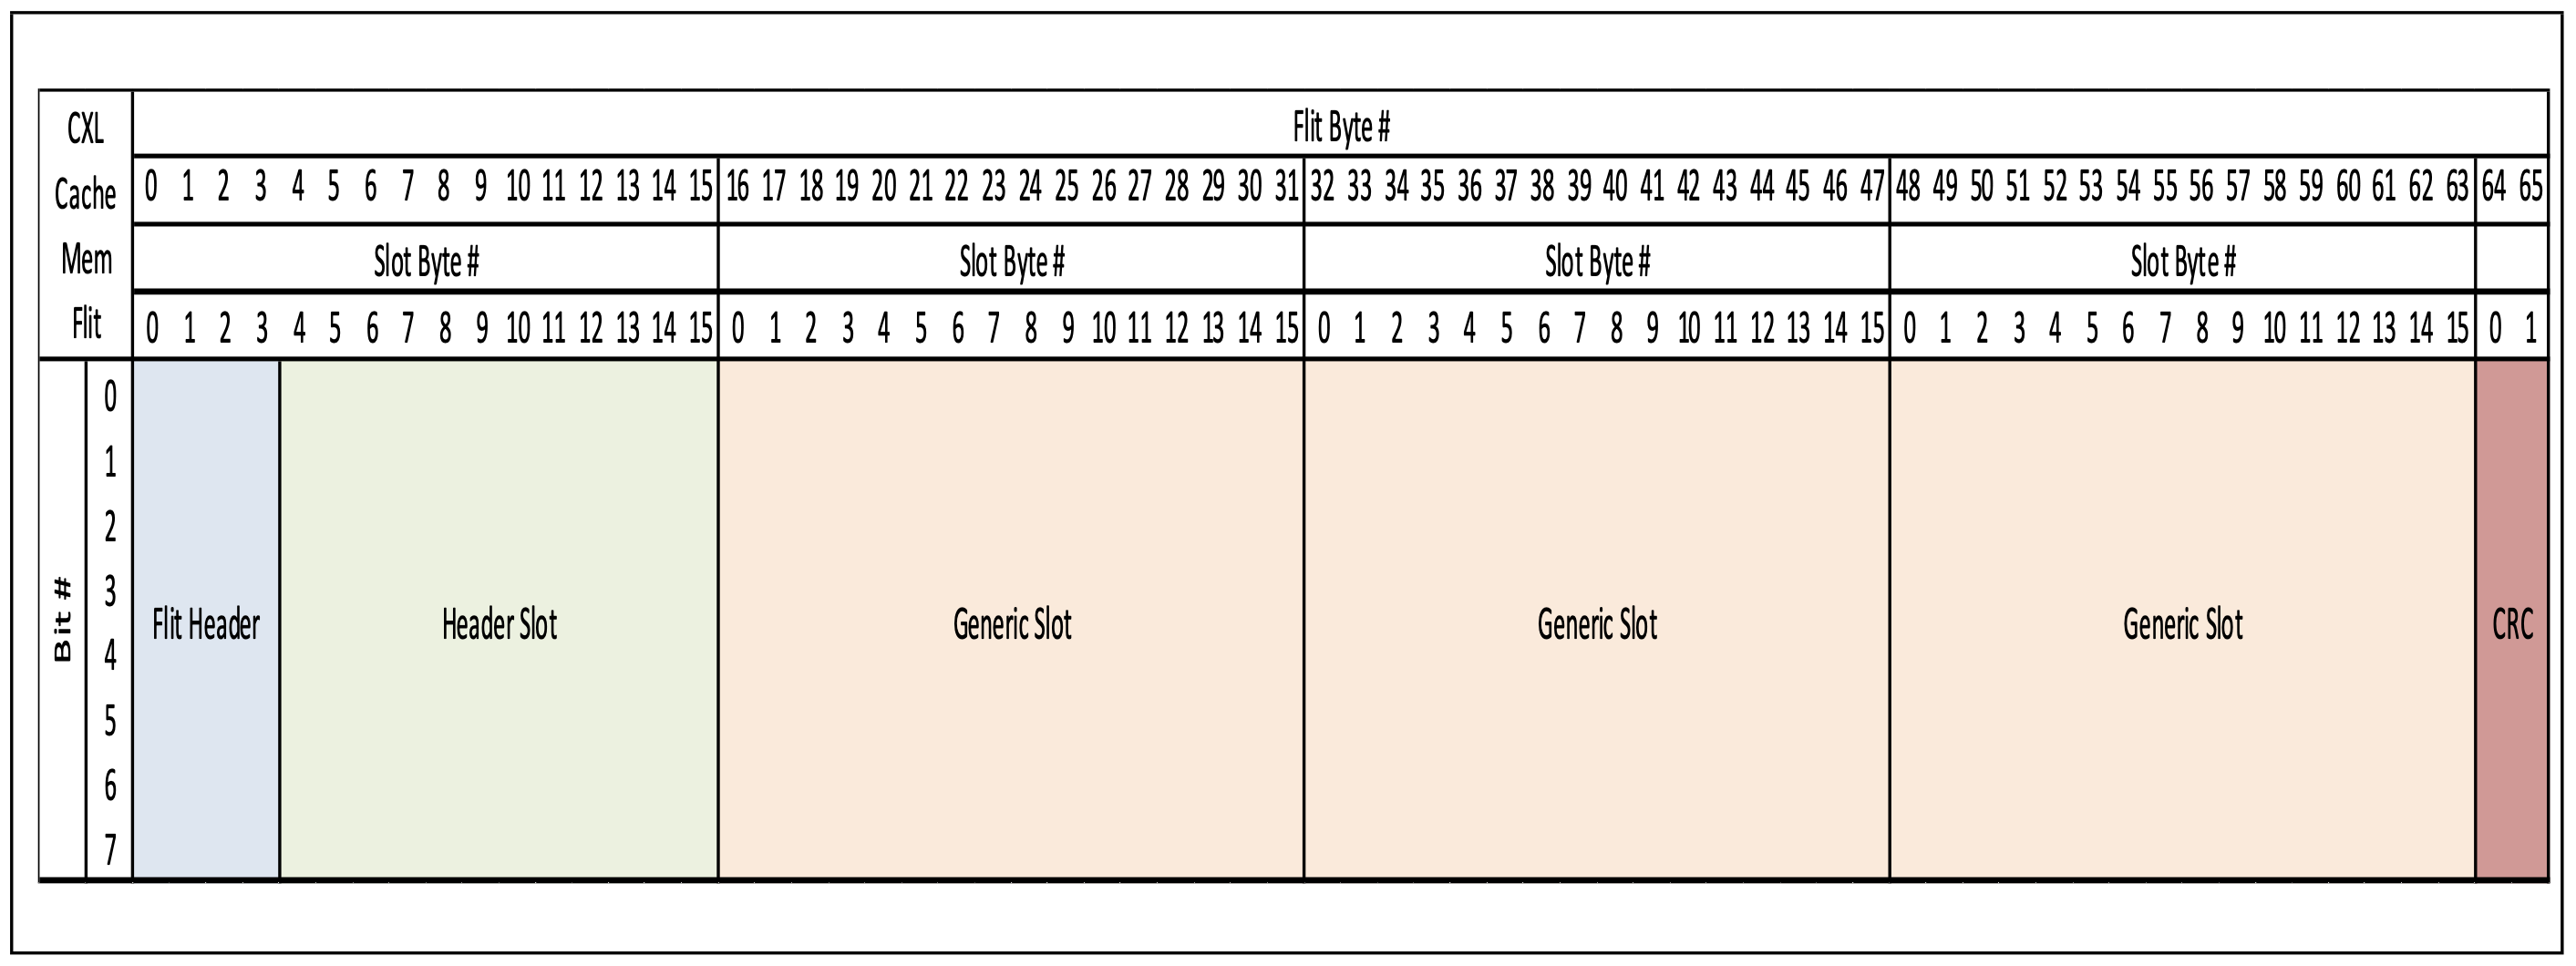
\includegraphics[width=\textwidth]{figures/flit.png}
  \caption{Flit with 1 header slot and 3 generic slots.}
  \label{fig:flit}
\end{figure}

\begin{figure}[ht]
  \centering
  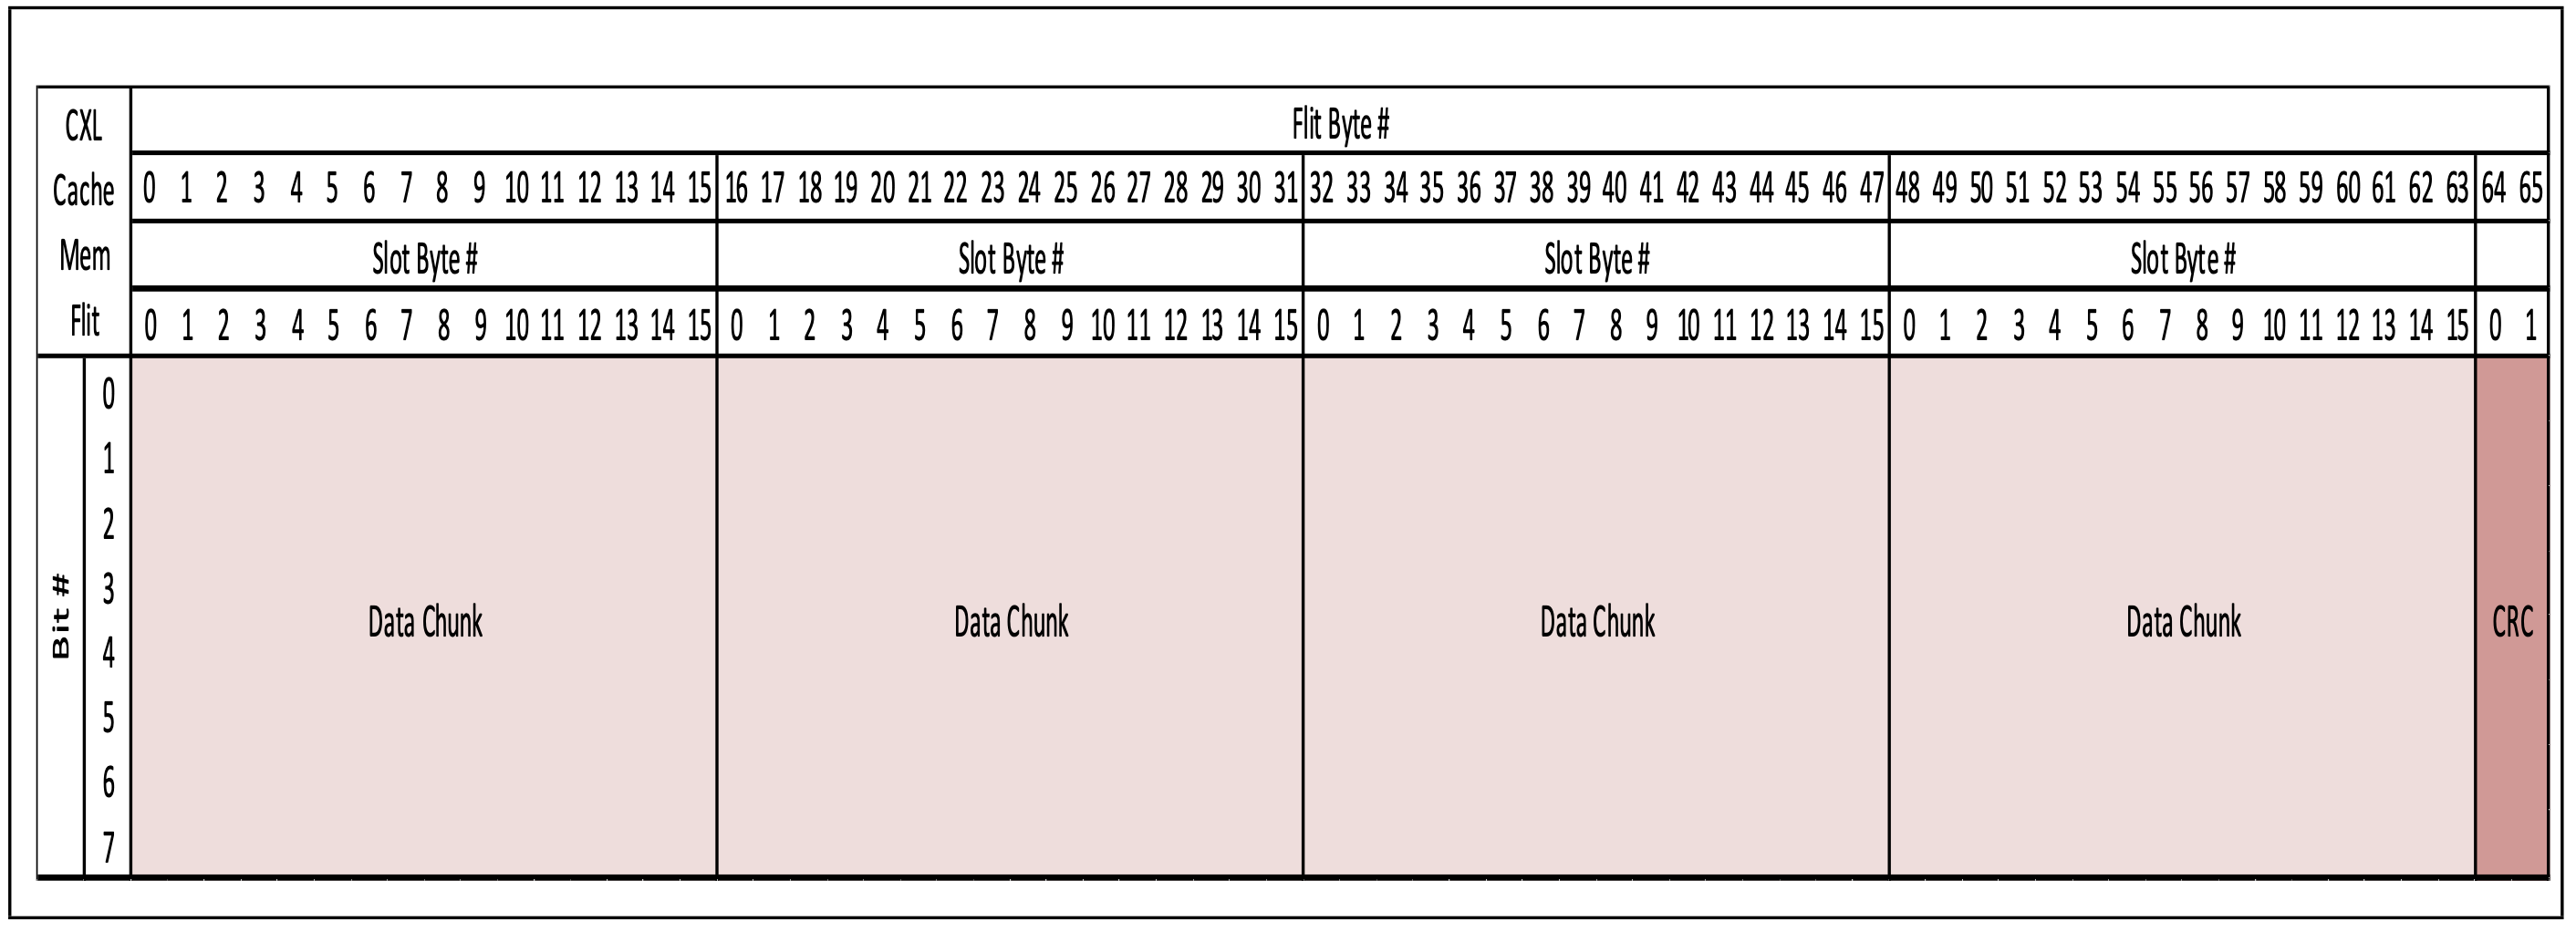
\includegraphics[width=\textwidth]{figures/all-data-flit.png}
  \caption{Flit with 4 data chunks.}
  \label{fig:all-data-flit}
\end{figure}

The 32 bit flit header in Figure \ref{fig:flit} contains format type information for each slot in the flit. As slot size (12 byte header slot, 16 byte generic slot) is larger than one message size (87 bit REQ, 87 bit RWD, 30 bit NDR, 40 bit DRS), each slot contains several messages. Therefore, there are rules to make header slot and generic slot. For example, in case of S2M transaction, header slot can have 2 DRS or 2 NDR or 1 DRS + 1 NDR. In case of generic slot, it can contain 3 DRS or 2 NDR or 1 DRS + 2 NDR or data chunk. This kind of details are explained in CXL specification \cite{CXL}. Other than slot making, there are some more flit packing policies such as data chunk rollover and number of messages per flit.